% =====================================================================
%  CP 320 Operations Research for Mobility Management -- Course Project
%  EV Charging Network Optimization
%  Yakshith Maddineni (SR 26080) and Kartikeya Gaur
%
%  Beamer (LaTeX) presentation.
%  Compile with:   pdflatex presentation.tex   (run twice)
%             or:  latexmk -pdf presentation.tex
%
%  Logos: put iisc_logo.(png|jpg|pdf) and system_logo.(png|jpg|pdf)
%         in the logos/ folder. Until then, dashed placeholders show.
% =====================================================================
\documentclass[aspectratio=169,11pt]{beamer}

% ---------- Theme base (plain, no font dependencies -> pdflatex safe) ----------
\usetheme{default}
\setbeamertemplate{navigation symbols}{}      % remove navigation clutter

% ---------- Encoding / fonts ----------
\usepackage[T1]{fontenc}
\usepackage[utf8]{inputenc}
\usepackage{lmodern}

% ---------- Math, tables, graphics ----------
\usepackage{amsmath,amssymb}
\usepackage{booktabs,array,tabularx}
\usepackage{graphicx}
\usepackage{tikz}
\usetikzlibrary{arrows.meta,positioning,calc}

% ---------- Project colours (match the written reports) ----------
\definecolor{headblue}{RGB}{38,70,120}        % primary
\definecolor{accent}{RGB}{199,120,20}         % warm accent (FCS drive)
\definecolor{accent2}{RGB}{30,120,90}         % teal-green (van route)
\definecolor{accent3}{RGB}{120,70,150}        % purple (resources)
\definecolor{lightblue}{RGB}{225,232,243}

% tiny reference / footnote line, placed at the foot of a frame
\newcommand{\refline}[1]{{\scriptsize\color{black!55}\raggedright #1\par}}
% one objective term: \zterm{Z_1}{formula}{gloss}
\newcommand{\zt}[2]{{\color{headblue}\bfseries #1}\ \ #2}

\setbeamercolor{structure}{fg=headblue}
\setbeamercolor{title}{fg=headblue}
\setbeamercolor{frametitle}{fg=headblue}
\setbeamercolor{itemize item}{fg=headblue}
\setbeamercolor{itemize subitem}{fg=accent}
\setbeamercolor{block title}{fg=white,bg=headblue}
\setbeamercolor{block body}{bg=lightblue!40}
\setbeamercolor{footsym}{fg=white,bg=headblue}
\setbeamercolor{alerted text}{fg=accent}

\setbeamertemplate{itemize item}{\small\raise0.3ex\hbox{\textbullet}}
\setbeamertemplate{itemize subitem}{\footnotesize\raise0.2ex\hbox{--}}

% ---------- Frame title: bold headblue with an underline rule ----------
\setbeamerfont{frametitle}{series=\bfseries,size=\large}
\setbeamertemplate{frametitle}{%
  \vspace{0.7em}%
  \hspace{0.3em}\usebeamercolor[fg]{frametitle}\insertframetitle\par%
  \vspace{-0.25em}\hspace{0.3em}{\color{headblue}\rule{0.965\paperwidth}{1.2pt}}%
}

% ---------- Footline: author  |  short title  |  frame number ----------
\setbeamertemplate{footline}{%
  \leavevmode%
  \begin{beamercolorbox}[wd=\paperwidth,ht=2.6ex,dp=1.1ex]{footsym}%
    \hbox to\paperwidth{%
      \hspace{1em}\scriptsize Yakshith \& Kartikeya%
      \hfill\scriptsize EV Charging Network Optimization\hfill%
      \scriptsize\insertframenumber\,/\,\inserttotalframenumber\hspace{1em}%
    }%
  \end{beamercolorbox}%
  \vskip0pt%
}

% =====================================================================
%  Logo helpers
% =====================================================================
\newcommand{\logoheight}{1.25cm}

% Dashed placeholder shown until a real logo file is dropped in logos/
\newcommand{\placeholderlogo}[1]{%
  \begin{tikzpicture}
    \node[draw=headblue,dashed,rounded corners=2pt,
          minimum height=\logoheight,minimum width=2.6cm,
          align=center,text=headblue,font=\scriptsize,inner sep=2pt]
      {#1 logo\\[-1pt]\textit{\tiny drop file in logos/}};
  \end{tikzpicture}%
}

% \showlogo{basename}{placeholder text}  -- looks in logos/ for pdf/png/jpg
\newcommand{\showlogo}[2]{%
  \IfFileExists{logos/#1.pdf}{\includegraphics[height=\logoheight]{logos/#1}}{%
   \IfFileExists{logos/#1.png}{\includegraphics[height=\logoheight]{logos/#1}}{%
    \IfFileExists{logos/#1.jpg}{\includegraphics[height=\logoheight]{logos/#1}}{%
     \placeholderlogo{#2}}}}%
}

% ---------- PDF metadata ----------
\hypersetup{pdftitle={EV Charging Network Optimization},
            pdfauthor={Yakshith Maddineni, Kartikeya Gaur}}

% =====================================================================
\begin{document}

% ---------------------------------------------------------------------
%  TITLE SLIDE
% ---------------------------------------------------------------------
\begin{frame}[plain]
  \centering

  % --- Logo (centred) ---
  \vspace{0.2em}
  {\showlogo{iisc_logo}{IISc}\par}

  \vspace{0.6em}

  % --- Course ---
  {\color{accent}\bfseries\large CP 320 \textbullet\ Operations Research for Mobility Management\par}
  \vspace{0.1em}
  {\footnotesize Course Project\par}

  \vspace{0.7em}

  % --- Project title ---
  {\color{headblue}\bfseries\huge EV Charging Network Optimization\par}
  \vspace{0.35em}
  {\color{black!75}\normalsize Assigning EV requests to fixed \& mobile chargers and\\[1pt]
   routing mobile charging vans \,--\, MILP and Reinforcement Learning\par}

  \vspace{0.6em}
  {\color{headblue}\rule{0.55\textwidth}{1pt}\par}
  \vspace{0.6em}

  % --- Authors ---
  {\large\bfseries Yakshith Maddineni\,\normalsize\ (SR No.\ 26080) \quad\textbullet\quad \large\bfseries Kartikeya Gaur\par}
  \vspace{0.15em}
  {\small M.Tech Smart Mobility \& Logistics Systems \,\textbullet\, Indian Institute of Science, Bengaluru\par}

  \vspace{0.45em}
  {\footnotesize Course Instructor:\ Prof.\ Prasant Misra, Dept.\ of Cyber Physical Systems\par}

  \vspace{0.7em}
  {\footnotesize\color{black!60} November 2026\par}
\end{frame}

% =====================================================================
%  ======  EVERYTHING BELOW IS A STARTER SCAFFOLD -- edit freely  ======
%  Add a \section{...} before a group of frames and it appears in the
%  Outline frame automatically. Duplicate a frame to add content.
% =====================================================================

% ---------------------------------------------------------------------
%  OUTLINE
% ---------------------------------------------------------------------
\begin{frame}{Outline}
  \tableofcontents
\end{frame}

%=====================================================================
\section{Problem and model}
%=====================================================================

% ---------- Problem ----------
\begin{frame}{The problem: EV charging assignment \& routing}
  \begin{itemize}
    \item During a period $[0,T]$, parked EVs raise charging requests; \textbf{every} request must be served.
    \item Two resources for each EV:
      \begin{itemize}
        \item a \textbf{fixed charging station} (FCS, 2 guns $\times$ 22\,kW) the car \emph{drives} to and queues at, or
        \item a \textbf{mobile charging van} (MCS) \emph{routed} from a depot that charges the car on the spot.
      \end{itemize}
    \item Every EV also carries a \textbf{segment} (personal / commercial) and an \textbf{income} $\theta\in[0,1]$, which set how it values money, time and queueing.
  \end{itemize}
  \vspace{0.3em}
  \begin{block}{Decide, to minimise operator cost $+$ perceived customer cost}
    \textbf{(1)} who serves each EV (a gun or a van)\quad\textbullet\quad
    \textbf{(2)} each van's route\quad\textbullet\quad
    \textbf{(3)} every charging start time.
  \end{block}
\end{frame}

% ---------- System model ----------
\begin{frame}{System model}
  \begin{columns}[T]
    \begin{column}{0.46\textwidth}
      \centering
      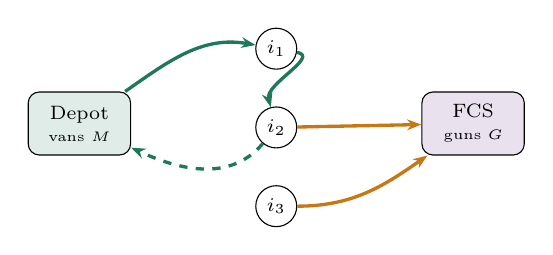
\begin{tikzpicture}[font=\scriptsize,>={Stealth[length=1.8mm]},
        box/.style={draw,rounded corners,align=center,minimum height=0.8cm,minimum width=1.3cm},
        ev/.style={circle,draw,fill=white,minimum size=0.52cm,inner sep=0pt}]
        \node[box,fill=accent2!14] (depot) at (0,0) {Depot\\{\tiny vans $M$}};
        \node[ev] (e1) at (2.5,0.95) {$i_1$};
        \node[ev] (e2) at (2.5,-0.05) {$i_2$};
        \node[ev] (e3) at (2.5,-1.05) {$i_3$};
        \node[box,fill=accent3!16] (fcs) at (5.0,0) {FCS\\{\tiny guns $G$}};
        \draw[->,accent2,very thick] (depot) to[out=35,in=170] (e1);
        \draw[->,accent2,very thick] (e1) to[out=-10,in=105] (e2);
        \draw[->,accent2,very thick,dashed] (e2) to[out=-130,in=-25] (depot);
        \draw[->,accent,very thick] (e2) -- (fcs);
        \draw[->,accent,very thick] (e3) to[out=0,in=215] (fcs);
      \end{tikzpicture}\\[4pt]
      {\scriptsize \textcolor{accent2}{\textbf{van}}: route from depot, charge in place\\
       \textcolor{accent}{\textbf{FCS}}: drive $+$ queue $+$ charge}
    \end{column}
    \begin{column}{0.54\textwidth}
      {\footnotesize
      \textbf{Decision variables}
      \begin{itemize}
        \item $y_{ig}$ EV $i$ at gun $g$;\ \ $z_{im}$ EV $i$ on van $m$ \ ($y_i+z_i=1$)
        \item $x_{ijm}$ van $m$ arc $i\!\to\!j$;\ \ $u_m$ van $m$ used
        \item $S_i$ charging start;\ \ $q^{\mathrm F}_i,q^{\mathrm M}_i$ FCS queue / van wait
        \item $C_i=S_i+\tau^{\mathrm F}_iy_i+\tau^{\mathrm M}_iz_i$ \ (completion)
      \end{itemize}
      \vspace{1pt}
      Charging time is physics: $\tau^{\mathrm F}_i=\tfrac{60E_i}{P^{\mathrm F}},\ \tau^{\mathrm M}_i=\tfrac{60E_i}{P^{\mathrm M}}$, $P^{\mathrm M}>P^{\mathrm F}$.}
      \vspace{3pt}
      \begin{block}{}
        {\footnotesize Solved \textbf{exactly} as a MILP (Gurobi) --- and that MILP is the \textbf{baseline} for the RL method.}
      \end{block}
    \end{column}
  \end{columns}
\end{frame}

% ---------- Objective Z1-Z6 ----------
\begin{frame}{Objective: six cost terms \ $Z=Z_1+\cdots+Z_6$}
  \begin{columns}[T]
    \begin{column}{0.57\textwidth}
      {\footnotesize
      \begin{align*}
        Z_1&=\textstyle\sum_i \mu_i\,c^{\mathrm{EV}}\!\sum_f d_{if}Y_{if}\\
        Z_2&=\textstyle c^{\mathrm M}\!\sum_m\sum_{(i,j)} d_{ij}x_{ijm}\\
        Z_3&=\textstyle\sum_m c^{\mathrm F}_m u_m\\
        Z_4&=\textstyle\pi^{\mathrm F}\!\sum_i E_i y_i+\pi^{\mathrm M}\!\sum_i\tfrac{E_i}{\eta}z_i\\
        Z_5&=\textstyle\sum_i \mu_i E_i(p^{\mathrm F}y_i+p^{\mathrm M}z_i)\\
        Z_6&=\textstyle\sum_i\!\big(c^{\mathrm D}_i t Y_{if}+c^{\mathrm Q}_i q^{\mathrm F}_i+c^{\mathrm C}_i\tau^{\mathrm F}_iy_i+c^{\mathrm V}_i(q^{\mathrm M}_i+\tau^{\mathrm M}_iz_i)\big)
      \end{align*}}
    \end{column}
    \begin{column}{0.43\textwidth}
      {\footnotesize
      \begin{block}{Operator cost $=Z_2+Z_3+Z_4$}
        van km, van dispatch, grid electricity
      \end{block}
      \begin{block}{Customer \emph{felt} cost $=Z_1+Z_5+Z_6$}
        felt driving \& tariff ($\times\mu_i$), and the value of lost time --- drive / queue / charge / van
      \end{block}
      \vspace{1pt}
      $\mu_i$ (money) and $c^a_i$ (time) are each a \textbf{line in income}, with its own slope per \textbf{segment}.}
    \end{column}
  \end{columns}
\end{frame}

% ---------- Constraints ----------
\begin{frame}{Constraints (complete model, every size)}
  {\footnotesize
  \begin{columns}[T]
    \begin{column}{0.5\textwidth}
      \textbf{Assignment}
      \begin{itemize}\item $y_i+z_i=1$ --- served by exactly one resource\end{itemize}
      \textbf{Station (continuous time)}
      \begin{itemize}
        \item start after request $+$ drive; wait $=q^{\mathrm F}_i+q^{\mathrm M}_i$
        \item $q^{\mathrm F}_i\le W_i\,y_i$ --- queue tolerance
        \item $C_i\le T$ --- hard deadline
        \item one EV per gun (disjunctive), gun-load cut, symmetry
      \end{itemize}
    \end{column}
    \begin{column}{0.5\textwidth}
      \textbf{Van routing}
      \begin{itemize}
        \item each van leaves \& returns once; flow conservation
        \item $\sum_i z_{im}\le Q_m u_m$ --- seats
        \item $\sum_i\tfrac{E_i}{\eta}z_{im}+\beta\!\sum d_{ij}x_{ijm}\le B_m u_m$ --- battery
        \item one EV at a time, no subtours, back by $T$
      \end{itemize}
      \textbf{Domains}
      \begin{itemize}\item binaries $y,z,x,u,o$;\ \ $S_i,q^{\mathrm F}_i,q^{\mathrm M}_i\ge0$\end{itemize}
    \end{column}
  \end{columns}}
  \vspace{3pt}
  \refline{23 constraints; the \emph{complete} formulation is solved for every instance (no reduced station, arc or neighbour sets).}
\end{frame}

%=====================================================================
\section{Reinforcement-learning method}
%=====================================================================

% ---------- RL representation + masking ----------
\begin{frame}{RL: build the plan as a sequence of decisions}
  \centering
  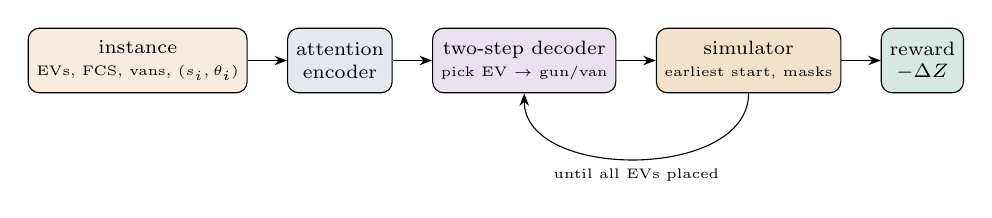
\begin{tikzpicture}[font=\scriptsize,>={Stealth[length=1.6mm]},
    b/.style={draw,rounded corners,align=center,minimum height=0.82cm,inner sep=3pt}]
    \node[b,fill=accent!14](inst){instance\\{\tiny EVs, FCS, vans, $(s_i,\theta_i)$}};
    \node[b,fill=headblue!12,right=5mm of inst](enc){attention\\encoder};
    \node[b,fill=accent3!16,right=5mm of enc](dec){two-step decoder\\{\tiny pick EV $\to$ gun/van}};
    \node[b,fill=accent!22,right=5mm of dec](sim){simulator\\{\tiny earliest start, masks}};
    \node[b,fill=accent2!18,right=5mm of sim](rew){reward\\$-\Delta Z$};
    \draw[->](inst)--(enc);\draw[->](enc)--(dec);\draw[->](dec)--(sim);\draw[->](sim)--(rew);
    \draw[->](sim.south) to[out=-90,in=-90] node[below,font=\tiny]{until all EVs placed}(dec.south);
  \end{tikzpicture}
  \vspace{3pt}
  {\footnotesize
  \begin{columns}[T]
    \begin{column}{0.5\textwidth}
      \textbf{State} $s_t$: unserved EVs; each gun's free time $a_g$; each van's position $\ell_m$, free time $a_m$, battery $b_m$, seats $\kappa_m$.\\[3pt]
      \textbf{Action} $(i,k)$: pick EV $i$, then resource $k$; the simulator schedules it at its \emph{earliest feasible} start.
    \end{column}
    \begin{column}{0.5\textwidth}
      \textbf{Mask} forbids any infeasible move:
      \begin{itemize}
        \item gun: in range, $q^{\mathrm F}\le W_i$, finish $\le T$
        \item van: seats left, battery enough, back by $T$
      \end{itemize}
      $\Rightarrow$ every finished episode is a \textbf{feasible plan}.
    \end{column}
  \end{columns}}
  \vspace{2pt}
  \refline{Encoder: Kool et al.\ 2019. \quad Two-step decoder: Li et al.\ 2021.}
\end{frame}

% ---------- Reward ----------
\begin{frame}{Reward $=$ the cost itself}
  {\footnotesize
  Reward of placing EV $i$ at resource $k$:\ \ $\boxed{\,r_t=-\Delta Z(i,k)\,}$\ \ (no discount).
  \begin{align*}
    \Delta Z(i,g)&=\underbrace{\mu_i c^{\mathrm{EV}}d_{if}}_{Z_1}+\underbrace{\pi^{\mathrm F}E_i}_{Z_4}+\underbrace{\mu_i p^{\mathrm F}E_i}_{Z_5}+\underbrace{c^{\mathrm D}_i t_{if}+c^{\mathrm Q}_i q^{\mathrm F}_i+c^{\mathrm C}_i\tau^{\mathrm F}_i}_{Z_6} &&\text{(gun)}\\[-1pt]
    \Delta Z(i,m)&=\underbrace{c^{\mathrm M}(\text{detour})}_{Z_2}+\underbrace{c^{\mathrm F}[\text{new van}]}_{Z_3}+\underbrace{\pi^{\mathrm M}\tfrac{E_i}{\eta}}_{Z_4}+\underbrace{\mu_i p^{\mathrm M}E_i}_{Z_5}+\underbrace{c^{\mathrm V}_i(q^{\mathrm M}_i+\tau^{\mathrm M}_i)}_{Z_6} &&\text{(van)}
  \end{align*}
  \begin{columns}[T]
    \begin{column}{0.54\textwidth}
      \begin{itemize}
        \item Return $\sum_t r_t=-Z$ of the plan $\Rightarrow$ \textbf{max return $\equiv$ min $Z$} (exact).
        \item Training minimises $\tilde c=Z+\lambda\sigma|D|$ ($\lambda=10$): a dropped EV costs $\sim$10 cars.
      \end{itemize}
    \end{column}
    \begin{column}{0.46\textwidth}
      \begin{itemize}
        \item \textbf{Normalised}: features scaled by $T$, battery $B$, typical cost $\sigma$ --- comparable across sizes.
        \item \textbf{Tie-breaks}: identical idle guns/vans $\to$ only the first offered; a \emph{busy} van $\to$ the EV waits ($q^{\mathrm M}$).
      \end{itemize}
    \end{column}
  \end{columns}}
\end{frame}

% ---------- Network ----------
\begin{frame}{Policy network: encoder--decoder attention}
  \relax{\footnotesize
  \begin{itemize}
    \item \textbf{Encoder} (multi-head self-attention, 3 layers, $d{=}128$, 8 heads): reads every EV, station and van with its features --- position, energy, request, \textbf{segment \& income} $(s_i,\theta_i)$ --- into one \textbf{embedding} per node.
      \begin{itemize}\item every node attends to every other, so an EV's embedding already carries its \emph{context} --- nearest stations, their costs, the fleet. Order-invariant $\Rightarrow$ one network works for any $n$.\end{itemize}
    \item \textbf{Two-step decoder}: step 1 scores the open EVs $\to$ pick EV $i$;\ \ step 2 scores the guns/vans for $i$ $\to$ pick resource $k$.
      \begin{itemize}\item each score $=$ learned vector $+$ the \emph{exact} current $\Delta Z(i,k)$, wait and finish; masked moves get probability $0$.\ \ $p(i,k)=p(i)\,p(k\mid i)$.\end{itemize}
    \item 765{,}858 learned weights.
  \end{itemize}}
  \vspace{2pt}
  \refline{Attention encoder: Kool, van Hoof \& Welling 2019. \quad Two-step (EV\,$\to$\,resource) decoder: Li et al.\ 2021.}
\end{frame}

% ---------- Training algorithm ----------
\begin{frame}{Training: REINFORCE with a shared baseline}
  {\footnotesize
  \begin{block}{Per epoch}
    \begin{flushleft}
    sample $B{=}32$ random instances (one size $n$); run the encoder once each\\
    play $S{=}8$ rollouts per instance by \emph{sampling} \ $\to$ \ $256$ episodes, costs $\tilde c_{bj}$\\
    baseline (POMO): \ $\bar c_b=\tfrac18\sum_j\tilde c_{bj}$ \ (mean of the 8 siblings)\\
    advantage: \ $A_{bj}=(\tilde c_{bj}-\bar c_b)/\bar c_b$\\
    loss: \ $\mathcal L=\tfrac{1}{BS}\sum_{b,j}A_{bj}\,\log p_\phi(\pi_{bj})$ \ ;\ \ Adam step (grad-clip 1.0)
    \end{flushleft}
  \end{block}
  \begin{itemize}
    \item Gradient $\nabla J=\mathbb E\big[(\tilde c-\bar c)\,\nabla\log p_\phi\big]$: a cheaper-than-average rollout gets its actions \emph{reinforced}; the shared baseline cuts variance with \textbf{no critic}.
    \item \textbf{Warm-up}: first 500 batches imitate a greedy rule; then REINFORCE. Min 200 epochs, early stop; lr $10^{-4}\!\to\!2\!\times\!10^{-5}$.
  \end{itemize}}
  \vspace{2pt}
  \refline{REINFORCE: Williams 1992. \quad Shared (POMO) baseline: Kwon et al.\ 2020.}
\end{frame}

% ---------- Worked example ----------
\begin{frame}{One episode, step by step (EV-C101, first $n=8$)}
  {\footnotesize Instance: $T=1236$\,min, 12 stations $\times$ 2 guns, 5 vans, typical cost $\sigma=916.8$\,Rs.}
  \vspace{3pt}
  {\footnotesize
  \begin{itemize}
    \item[$t_1$] \textbf{Stranded car first} (no station in range) $\to$ \textbf{van 1}, $p=1.00$.\ \ $\Delta Z=2287$\,Rs (incl.\ 1500 dispatch). The van leaves the depot and charges it on the spot.
    \item[$t_3$] \textbf{Rich private owner} ($\theta=0.82$) $\to$ the same \textbf{van 1}, $p=0.95$. The \emph{driver-free} benefit ($+313$\,Rs) beats the van premium ($+147$) and dearer energy ($+69$); a \emph{new} van would add 1500 dispatch $\to p=0$.
    \item[rest] the commercial cars go to the \textbf{nearest stations}, no queue.
  \end{itemize}}
  \vspace{1pt}
  \begin{block}{}
    {\footnotesize $\sum_t\Delta Z=$ checker $Z=7251.9$\,Rs (one greedy rollout). Best of \textbf{520} tries $=7208.8$\,Rs, only \textbf{0.02\%} above the MILP optimum (7207.2\,Rs, 0.39\,s).}
  \end{block}
\end{frame}

%=====================================================================
\section{Results and analysis}
%=====================================================================

% ---------- Evaluation ----------
\begin{frame}{Evaluation: one neutral yardstick}
  \begin{columns}[T]
    \begin{column}{0.54\textwidth}
      {\footnotesize
      \begin{itemize}
        \item One \textbf{independent checker} re-tests every constraint and recomputes $Z$ for \emph{all} plans (MILP, greedy, RL) --- no method reports its own cost.
        \item \textbf{Why this approach}: $\sim$0.12\,s vs $\sim$150\,s; finds plans where the MILP's 300\,s found none; reproduces the MILP's effects.
        \item \textbf{Self-check}: directions the optimiser \emph{cannot} break hold with \textbf{0 violations} in $\sim$4000 optimal pairs; MILP and RL agree within $\sim$0.15 pt.
      \end{itemize}}
    \end{column}
    \begin{column}{0.46\textwidth}
      \centering
      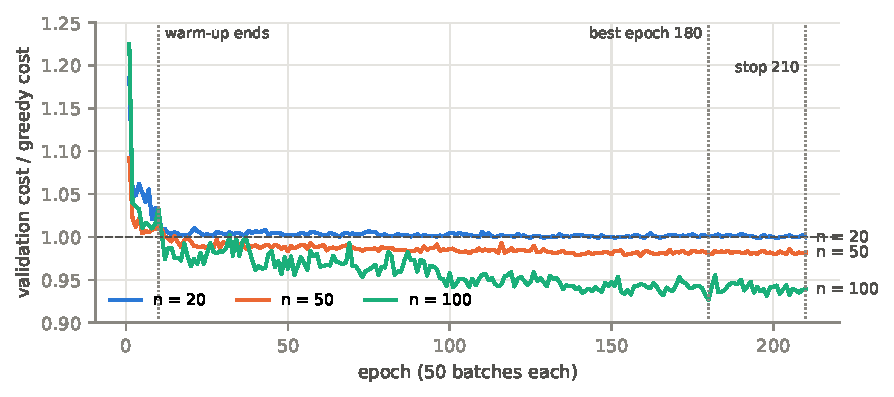
\includegraphics[width=\linewidth]{figures/rl_training.pdf}\\[2pt]
      {\scriptsize Training: validation cost vs the greedy rule, by size.}
    \end{column}
  \end{columns}
\end{frame}

% ---------- Results ----------
\begin{frame}{Results: exact (MILP) vs learned (RL)}
  \begin{columns}[T]
    \begin{column}{0.5\textwidth}
      {\footnotesize
      \textbf{MILP} (Gurobi, full model, 300\,s, 32 cores)
      \begin{itemize}
        \item 277/560 \textbf{proven optimal}, 474 valid plans
        \item 51 \textbf{proven infeasible} --- from the data (time, range, fleet), not the model
        \item mean 150.7\,s / instance
      \end{itemize}
      \textbf{RL} (attention policy)
      \begin{itemize}
        \item \textbf{500 valid} ($+26$ where the MILP found no plan)
        \item mean \textbf{0.85\%} above the MILP, \textbf{0.12\,s} ($\sim$1000$\times$)
      \end{itemize}}
    \end{column}
    \begin{column}{0.5\textwidth}
      \centering
      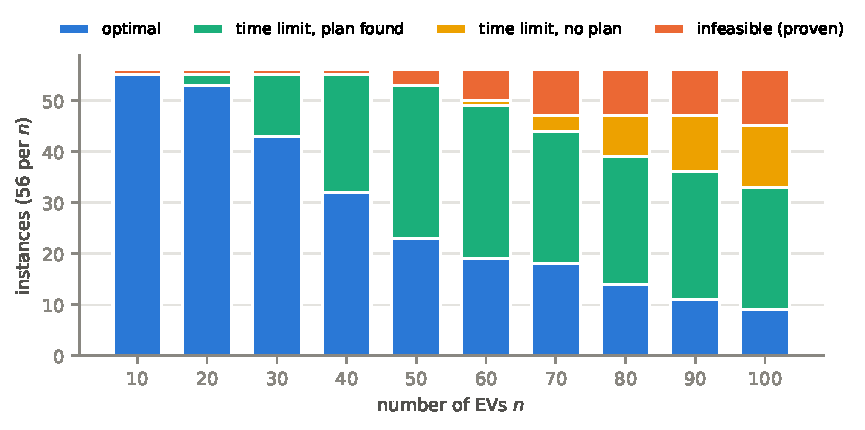
\includegraphics[width=\linewidth]{figures/milp_status_by_n.pdf}\\[2pt]
      {\scriptsize How the 560 instances end, by size.}
    \end{column}
  \end{columns}
  \vspace{2pt}
  \refline{Per instance the RL solve plays \textbf{8 map views $\times$ (1 greedy $+$ 64 sampled) $=$ 520 plans}, keeping the fewest-dropped then lowest-$Z$ plan.}
\end{frame}

% ---------- Analysis I: income & segment ----------
\begin{frame}{Analysis I --- who gets a van: income \& segment}
  \begin{columns}[T]
    \begin{column}{0.5\textwidth}
      {\footnotesize
      \begin{itemize}
        \item Vans go to \textbf{rich personal} owners: $\sim$20\% of free-choice personal cars (MILP) vs almost no commercial cars.
        \item Personal van use \textbf{climbs with income}: $0$\% below $\theta{=}0.4$ to $\sim$41\% above $0.8$.
        \item A taxi gains no driver-free benefit $\to$ takes a van \textbf{only to escape a queue} (congestion, not income).
        \item RL reproduces the \emph{pattern} but opens fewer vans ($6.7$\%), so the exact van policy is read from the MILP.
      \end{itemize}}
    \end{column}
    \begin{column}{0.5\textwidth}
      \centering
      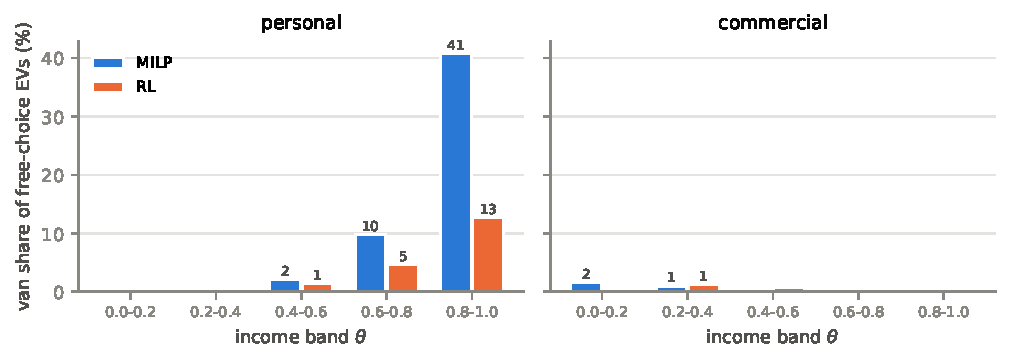
\includegraphics[width=\linewidth]{figures/van_share_income.pdf}\\[2pt]
      {\scriptsize Van share of free-choice cars, by segment \& income band.}
    \end{column}
  \end{columns}
\end{frame}

% ---------- Analysis II: demand & levers ----------
\begin{frame}{Analysis II --- demand \& the biggest levers}
  \begin{columns}[T]
    \begin{column}{0.5\textwidth}
      {\footnotesize
      \textbf{Demand pressure} $=$ charging work that must fit in the horizon $T$:
      \begin{itemize}
        \item \textbf{high} --- short-period classes R1/RC1 ($\sim$230\,min): long queues, some infeasibility;
        \item \textbf{low} --- long-period C2 ($\sim$3390\,min): ample time.
      \end{itemize}
      Charging demand itself: $\pm25\%$ energy $\to\pm22\%$ $Z$ (elasticity 0.88).\\[3pt]
      Biggest cost levers: energy \& station power, then \textbf{commercial money sensitivity} ($\pm6.4\%$); the \textbf{van tariff} sets \emph{who} gets a van.}
    \end{column}
    \begin{column}{0.5\textwidth}
      \centering
      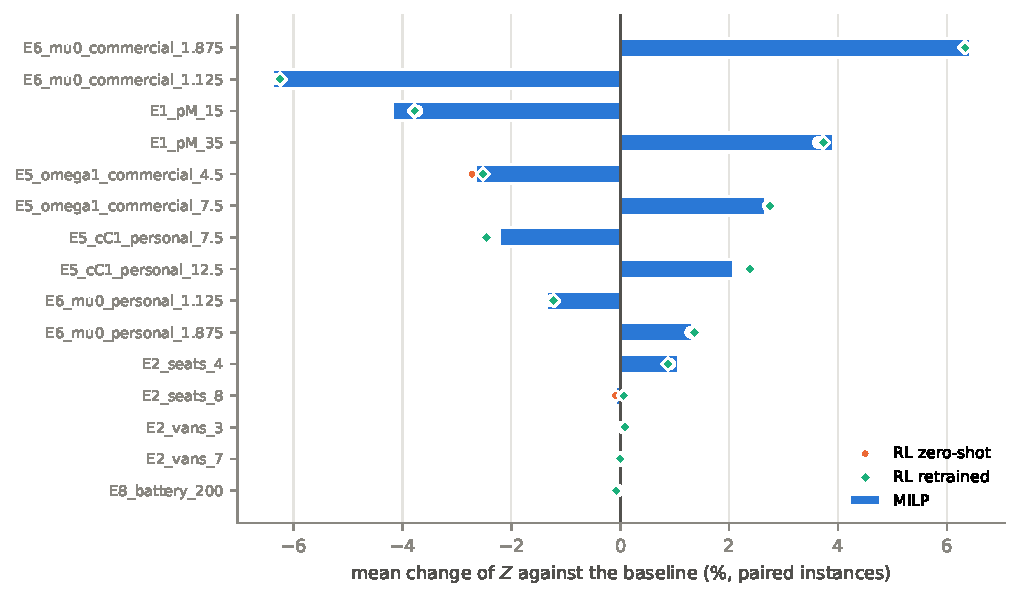
\includegraphics[width=\linewidth]{figures/exp_tornado.pdf}\\[2pt]
      {\scriptsize Effect on total cost $Z$ of a $\pm25\%$ change, by factor.}
    \end{column}
  \end{columns}
\end{frame}

%=====================================================================
\section{Summary}
%=====================================================================

% ---------- Summary ----------
\begin{frame}{Summary}
  {\footnotesize
  \begin{itemize}
    \item \textbf{What we built}: one optimisation that \emph{assigns} every EV to a fixed or mobile charger and \emph{routes} the vans, minimising operator $+$ perceived-customer cost --- for a network operator, \textbf{income- and segment-aware}.
    \item \textbf{Novelty}: a continuous income index $\theta$ and a personal/commercial segment set each customer's money and time valuation; a van's charging is priced \emph{driver-free} for private cars but as \emph{downtime} for taxis.
    \item \textbf{Two methods, one checker}: an exact MILP (Gurobi) as ground truth and an \textbf{attention policy} (REINFORCE\,+\,POMO) as a fast learned solver; benchmarked against a greedy rule and a 520-plan search.
    \item \textbf{Behavioural insight}: vans are a \emph{premium service for rich private owners}; \emph{queues, not income}, push taxis to vans.
  \end{itemize}}
\end{frame}

% ---------- Conclusion ----------
\begin{frame}{Conclusion}
  {\footnotesize
  \begin{itemize}
    \item \textbf{Segment, not income, decides van use} (rules T1--T3), and it holds across every experiment.
    \item \textbf{Technical (RL)}: setting the reward to $-\Delta Z$ makes the return exactly $-Z$, so a 766k-parameter attention policy trained with REINFORCE\,+\,POMO matches the exact optimum within \textbf{0.85\%} at $\sim$1000$\times$ the speed --- and even solves instances the MILP could not in 300\,s.
    \item \textbf{Trustworthy}: two independent methods agree to a fraction of a per cent, and every provable direction holds with \textbf{0 violations}.
  \end{itemize}}
\end{frame}

% ---------- Future work ----------
\begin{frame}{Future work}
  {\footnotesize
  \begin{itemize}
    \item \textbf{Beyond REINFORCE}: the learner is a Monte-Carlo, full-episode policy gradient with a shared (POMO) baseline. Natural next steps are \textbf{actor--critic} and \textbf{PPO} --- a learned critic and clipped updates for lower-variance, step-level credit (the shared baseline already points that way).
    \item \textbf{Richer problem}: \emph{dynamic} demand (requests arriving through the day, not all at $t=0$), \emph{equity} as an explicit objective, and multi-factor experiments (price\,$\times$\,fleet, demand\,$\times$\,power).
    \item Van recharging can stay out of the model (its effect is $\approx0\%$).
  \end{itemize}}
  \vspace{4pt}
  \centering {\color{headblue}\bfseries Thank you \quad\textbullet\quad Questions?}
\end{frame}

\end{document}
